\RequirePackage{docswitch}
\setjournal{\flag}

\documentclass[\docopts]{\docclass}


\usepackage{lsstdesc_macros}

\usepackage{xspace}
\usepackage{graphicx}
\graphicspath{{./}{./figures/}{.logos}}
\bibliographystyle{apj}


\newcommand{\textul}{\underline}
\newcommand{\qp}{\texttt{qp}}
\newcommand{\pz}{photo-$z$ PDF}
\newcommand{\Pz}{Photo-$z$ PDF}
\newcommand{\mgdata}{bright\xspace}
\newcommand{\Mgdata}{Bright\xspace}
\newcommand{\ssdata}{faint\xspace}
\newcommand{\Ssdata}{Faint\xspace}


\begin{document}

\title{ Approximating photo-z PDFs for large surveys }


\begin{abstract}

Modern galaxy surveys produce redshift probability distribution functions 
(PDFs) in addition to traditional photometric redshift (photo-$z$) point 
estimates.
However, the storage of \pz s may present a challenge with increasingly large 
catalogs, as we face a trade-off between the accuracy of subsequent science 
measurements and the limitation of finite storage resources.
This paper presents \qp, a Python package for manipulating parametrizations of 
1-dimensional PDFs, as suitable for \pz\ compression.
We use \qp\ to investigate the performance of three simple PDF storage formats 
on two realistic mock datasets, representative of upcoming surveys with 
different data qualities.
Based on metrics of individual \pz s and an estimator of the overall redshift 
distribution function, as an example of a science use case, as a function of 
the number of stored parameters per \pz, we make recommendations for best 
practices in choosing \pz\ approximation schemes.

\end{abstract}

\dockeys{methods: statistical, methods: miscellaneous, astronomical databases: 
miscellaneous, catalogs, galaxies: distances and redshifts}

\maketitlepost


\section{Introduction}
\label{sec:intro}


Upcoming wide-field imaging surveys such as the Large Synoptic Survey Telescope 
(LSST)\footnote{\url{https://www.lsst.org/}}\citep{ivezic_lsst:_2008} will 
observe tens of billions of galaxies photometrically, without follow-up 
spectroscopy.
Over the past decade, the Kilo-Degree 
Survey\footnote{\url{http://kids.strw.leidenuniv.nl/}}, Hyper Suprime-Cam 
Subaru Strategic Program\footnote{\url{http://hsc.mtk.nao.ac.jp/ssp/}}, and 
Dark Energy Survey\footnote{\url{https://www.darkenergysurvey.org/}} have paved 
the way for LSST via similar survey strategies on tens of millions of galaxies.
Studies of precision cosmology and galaxy evolution with the anticipated data 
will thus rely almost exclusively on the method of photometric redshift 
(photo-$z$) estimation.
Photo-$z$s are subject to a number of systematic errors, some caused by the 
estimation procedures and others intrinsic to the data itself.
For the purpose of producing public photo-$z$ catalogs, the redshift estimation 
community has thus come to favor methods that provide a photo-$z$ probability 
distribution function (PDF) conveying the potential for such systematic errors 
for each galaxy in the survey \citep{tanaka_photometric_2017, jong_third_2017, 
sheldon_photometric_2012}.

Given that the \pz\ catalogs of ongoing surveys already include $\sim10^{7}$ 
galaxies, and that those of upcoming surveys will include $\sim10^{10}$ 
galaxies, storage of these probability distributions must balance of accuracy 
of the catalog against limited storage resources.
For example, the public catalog that LSST will release will be limited to 
$\sim100$ floating point numbers per galaxy for all redshift information 
\citep[Section 4.2.2]{juric_data_2017}, with plans to store \pz s derived by 
multiple methods.
Furthermore, the problem of storing PDFs is not unique to galaxy surveys.
Gaia\footnote{\url{https://www.gaia-eso.eu/}}, for example, has committed to 
providing a catalog of PDFs of stellar properties inclding velocities, so an 
approach to optimizing the choice of PDF storage parametrization could benefit 
astronomy more broadly.

\citet{carrasco_kind_sparse_2014} first addressed the question of approximating 
\pz s in the context of a single galaxy survey and metrics applicable to 
deterministic, not probabilistic, data products.
However, we expect the optimal choice of \pz\ storage approximation to depend 
on the intended science applications and their requirements on \pz\ accuracy 
and the properties of the anticipated \pz s.
Different science cases will need different metrics, and different formats may 
be appropriate for different datasets.
In this paper, we address the question of \textit{how} these choices should be 
made, by providing the publicly available \qp\ Python 
package\footnote{\url{https://github.com/aimalz/qp}} enabling each survey to 
optimize their \pz\ approximation via mathematically motivated and 
science-driven metrics.
We demonstrate this approach on two sets of realistic mock data in the context 
of LSST.

In Section~\ref{sec:methods}, we outline how \qp\ can be used to optimize the 
choice of \pz\ parametrization.
In Section~\ref{sec:data}, we describe the mock datasets on which we 
demonstrate such an analysis.
We present the results of this procedure in Section~\ref{sec:results} and make 
recommendations for the use of \qp\ by the photo-$z$ community in 
Section~\ref{sec:conclusions}.

\section{Methods}
\label{sec:methods}


We have developed the \qp\ Python package to facilitate the approximation of 
one-dimensional PDFs, including \pz s, and comparisons between approximations.
A \texttt{qp.PDF} object is associated with sets of parameters for each 
approximation considered.
Conversions between approximations are facilitated by the 
\texttt{numpy}\footnote{\url{http://www.numpy.org/}}, \texttt{scipy} 
\footnote{\url{https://www.scipy.org/}}, and 
\texttt{scikit-learn}\footnote{\url{http://scikit-learn.org}} 
\citep{pedregosa_scikit-learn:_2011} tools.
The currently supported parametrizations are described in 
Section~\ref{sec:approx}.

The \qp\ package also provides a few built-in metrics for the accuracy of a 
representation of a PDF relative to a given reference representation.
Built-in plots are made using 
\texttt{matplotlib}\footnote{\url{https://matplotlib.org/}}.
A subset of the included metrics are described in Section~\ref{sec:metric}.

Catalog-level manipulations are performed using the \texttt{qp.Ensemble} class 
that serves as a wrapper for operations over collections of \texttt{qp.PDF} 
objects.
Parallelization is facilitated by the \texttt{pathos} 
\footnote{\noindent\url{http://trac.mystic.cacr.caltech.edu/project/pathos/wiki.
html}} \citep{mckerns_building_2012, mckerns_pathos:_2010} package.

\subsection{Approximation Methods}
\label{sec:approx}

First, we establish a vocabulary for the approximations.
Each \textit{parametrization} of a \pz\ is defined in terms of the 
\textit{parameters} $\vec{c}$ unique to its catalog entry, the 
\textit{metaparameters} $\vec{C}$ shared over the whole catalog, and the 
\textit{format} function $\mathcal{F}$ that reconstructs a PDF from its 
parameters and metaparameters.
A parametrization in turn corresponds to a \textit{representation}
\begin{align}
  \label{eq:definition}
  \hat{p}^{\mathcal{F}, \vec{C}, \vec{c}}(z) &\equiv \mathcal{F}_{\vec{C}}(z; 
\vec{c})
\end{align}
of the approximated \pz, denoted as $\hat{p}(z)$ for brevity.
The \textit{dimensionality} of $\vec{c}$ is the number $N_{f}$ of stored 
parameters per \pz, which are presumed to be scalar numbers unless otherwise 
specified.
The number of elements of $\vec{C}$ is of little importance so long as the 
metaparameters can be stored outside the catalog entries.

\qp\ currently supports conversion of \pz\ approximations between five formats: 
step functions, samples, quantiles, evaluations, and mixtures of 
\texttt{scipy.rv\_continuous} objects.
When the format function is not specified by the approximation, we refer to a 
generic interpolator function $F_{\vec{C}'}(z; \vec{c}, \mathcal{F}_{\vec{C}})$ 
with its own metaparameters $\vec{C}'$, which must be chosen by the researcher.
\qp\ supports numerous interpolation schemes, including several from the 
popular \texttt{scipy.interpolate} library.

In this work we consider special cases of three of these formats as candidates 
for large survey \pz\ catalog storage: regular binning 
(Section~\ref{sec:bins}), random samples (Section~\ref{sec:samples}), and 
regular quantiles (Section~\ref{sec:quantiles}).
These formats are illustrated on a multimodal PDF in Figure~\ref{fig:qp}.
\begin{figure}
  \begin{center}
    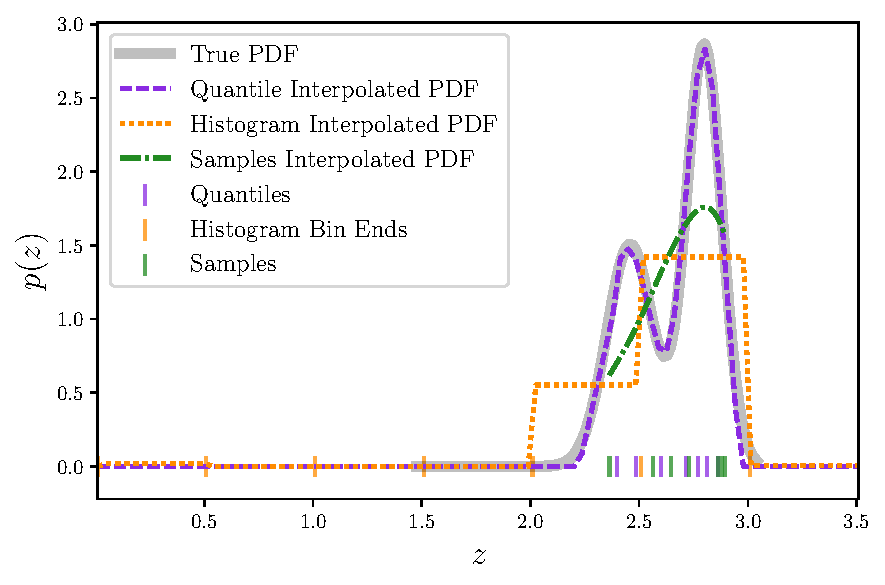
\includegraphics[width=\columnwidth]{figures/demo_pz.pdf}
    \caption{\qp\ approximation of a continuous 1-dimensional PDF (thick, solid 
gray line) using: the step function (orange dotted line), samples (green 
dash-dotted line), and quantile formats (purple dashed line) with the same 
number of stored parameters ($N_{f}=7$ in this case).
    \label{fig:qp}}
  \end{center}
\end{figure}

In spite of its impressive compression properties, we have not yet included the 
\texttt{SparsePz}\footnote{\url{https://github.com/mgckind/SparsePz}} sparse 
basis representation of \citet{carrasco_kind_sparse_2014}, in which the 
parameters are the integer identifiers of $N_{f}$ mixture model components from 
a library of $\sim10^{4}$ functions.
We omit this format because decomposition with \texttt{SparsePZ} does not 
enforce the condition that the representation be a probability distribution in 
the mathematical sense of nonnegativity and integration to unity.
While normalizing the integral of a positive semidefinite function is always 
possible (if the endpoints of integration are specified), one can motivate 
multiple schemes for enforcing nonnegativity that result in different 
reconstructions $\hat{p}(z)$.
We postpone to future work the exploration of adaptations of non-positive 
semidefinite representations and inclusion of the sparse basis representation 
in \qp.

For each format, we address the following questions:
\begin{itemize}
  \item When/where has the format appeared as a published catalog format, 
native \pz\ code output format, and science application input format?
  \item What exactly is stored under the format, per galaxy (the parameters) 
and per catalog (the metaparameters)?
  \item What are the a priori strengths and weaknesses of the format?
\end{itemize}

\subsubsection{Regular Binning}
\label{sec:bins}

By far the most popular format for approximating and storing \pz s is the 
piecewise constant step function, also called a histogram binning.
It is the native output of a number of \pz\ codes 
\citep{carrasco_kind_somz:_2014, sadeh_annz2:_2016, cavuoti_metaphor:_2017} and 
the only format that has been used for public release of \pz\ catalogs 
\citep{sheldon_photometric_2012, tanaka_photometric_2017, jong_third_2017}.

The metaparameters of the binned parametrization are the ordered list of 
redshifts $\vec{C} = (z_{1}, z_{2}, \dots, z_{N_{f}}, z_{N_{f}+1})$ serving as 
bin endpoints shared by all galaxies in the catalog, each adjacent pair of 
which is associated with a parameter $c_{i} = \int_{C_{i}}^{C_{i+1}} p(z) dz$.
The \qp\ histogram format assumes $p(z)=0$ when $z<C_{1}$ or $z>C_{N_{f}+1}$ 
and enforces the normalization condition\footnote{
Note that this is not generally equivalent to the erroneous normalization 
condition $\sum_{i} c_{i} = 1$ commonly enforced in public catalogs such as the 
Sloan Digital Sky Survey's Data Release 8 \citep{sheldon_photometric_2012}.
Unless redshift is treated as a discrete variable, the oversimplified 
normalization condition only holds if $C_{N_{f}+1} - C_{1} = N_{f} (C_{i+1} - 
C_{i})$ for all $i$ (under a regular binning).
}
\begin{align}
  \label{eq:normed}
  \sum_{i} c_{i} (C_{i+1} - C_{i}) &= 1.
\end{align}
The histogram format function $\mathcal{F}^{h}$ is thus the sum of a set of 
$N_{f}$ step functions, making the reconstructed estimator of the \pz
\begin{align}
  \label{eq:binned}
  \hat{p}^{h}(z) &= \sum_{i=1}^{N_{f}}\ c_{i} 
\left\{\begin{tabular}{cc}$1$&$C_{i}<z<C_{i+1}$\\
0&$z < C_{i}$\ or\ $z > C_{i+1}$\end{tabular}\right\},
\end{align}
where the step functions may be considered their own interpolators.
Though \qp\ supports arbitrary bin ends, here we only consider a regular 
binning, with $C_{i+1} = C_{i} + \delta$ for a constant $\delta = (C_{N_{f}+1} 
- C_{1}) / N_{f}$, as no irregular binning has yet been used for a public 
catalog of \pz s.

In terms of performance as a \pz\ storage format, we should anticipate the 
regular histogram format to be wasteful in terms of information content; a \pz\ 
with a very broad (compact) probability distribution may have many parameters 
taking the same value $c_{i} \approx (C_{N_{f}+1} - C_{1}) / \delta$ 
($c_{i}\approx0$) that are redundant in storage.
Additionally, we should expect the fidelity of $\hat{p}^{h}(z)$ to depend 
strongly on the bin widths relative to the sizes of and distances between 
features in the \pz s.

\subsubsection{Random Samples}
\label{sec:samples}

Samples are often the native output format of machine learning algorithms due 
to the discrete nature of training sets \citep{de_vicente_dnf_2016}.
Such approaches by default typically produce large numbers of samples, far more 
than can realistically be stored by any survey, so are commonly compressed by 
subsampling\citep{hoyle_dark_2017}.
Samples are easy to use in standard science applications developed for redshift 
point estimates, so they have an established presence in the 
literature\citep{bonnett_redshift_2016}.
The samples format of PDF storage appears elsewhere in astronomy, including the 
Gaia-ESO Survey's commitment to provide multi-dimensional PDFs of stellar 
parameters in the samples format \citep{bailer-jones_gaia_2013}.

The parameters of the samples format are the $N_{f}$ samples $\vec{c}=(z_{1}, 
z_{2}, \dots, z_{N_{f}-1}, z_{N_{f}})$, where $C=N_{f}$ is an implicit 
metaparameter.
Though it is possible to construct a catalog where $N_{f}$ is not uniform over 
the catalog, but is instead somehow optimized for each galaxy, we leave its 
investigation to future work, as it has not yet appeared in the literature.
The format function $\mathcal{F}^{s}$ that turns samples into a representation 
of the \pz\ is simply the interpolator $F$.
In the tests presented here, we use the Gaussian kernel density estimate (KDE) 
of \texttt{scipy.stats.gaussian\_kde}.
The samples representation is then
\begin{align}
  \label{eq:sampled}
  \hat{p}^{s}(z) &= \mathrm{KDE}_{C'}(z; \vec{c}).
\end{align}

Though samples are an obvious choice for \pz s with narrow features of high 
amplitude, we expect that using a small number of samples from a broad \pz\ may 
increase the variance of any ensemble metrics, as the sampling introduces 
additional shot noise.
The researcher must also choose an interpolation method to reconstruct a \pz\ 
from samples.

\subsubsection{Regular Quantiles}
\label{sec:quantiles}

One parametrization that has not previously been investigated in the context of 
photometric redshifts is that of quantiles, though they have appeared elsewhere 
in the astronomy literature \citep{sun_star_2015, pizzocaro_results_2016, 
laycock_x-ray_2017}.
The quantiles are defined in terms of the cumulative distribution function 
(CDF), which is the antiderivative of the PDF.

Under the quantile format, a \pz\ catalog shares $N_{f}$ ordered CDFs $\vec{C} 
= (q_{1}, q_{2}, \dots, q_{N_{f}-1}, q_{N_{f}})$ where $0 < q_{i} < 1$ for all 
$i$.
In this study, we test regular quantiles $C_{i} \equiv i / (N_{f} + 1)$.
Each galaxy's catalog entry is the vector of redshifts $\vec{c} = (z_{1}, 
z_{2}, \dots, z_{N_{f}-1}, z_{N_{f}})$ satisfying $\mathrm{CDF}(c_{i}) = 
C_{i}$, so the quantile format function $\mathcal{F}^{q}$ is the derivative of 
an interpolation $F$ of the CDF.
Our interpolator $F$ in the tests presented here is a nonnegative 
\texttt{scipy.interpolate} spline at $z_{1} \leq z \leq z_{N_{f}}$ and linear 
extrapolation subject to the normalization conditions of $\vec{C}$ elsewhere.
The quantile representation is thus
\begin{align}
  \label{eq:quantiles}
  \hat{p}^{q}(z) &=
  \left\{
  \begin{tabular}{cc}
  $\frac{d}{dz} \left[F(z; \vec{c}, \mathcal{F}^{q}_{\vec{C}})\right]$ & $c_{1} 
\leq z \leq c_{N_{f}}$ \\
  $\hat{p}^{q}(c_{1})\left(\frac{\hat{p}^{q}(c_{1})}{2C_{1}} z - 1\right)$ & $z 
< c_{1}$ \\
  $\hat{p}^{q}(c_{N_{f}})\left(1 - \frac{\hat{p}^{q}(c_{N_{f}})}{2(1 - 
C_{N_{f}})} z\right)$ & $z > c_{N_{f}+1}$
  \end{tabular}
  \right\}.
\end{align}


The quantile parametrization (the namesake of the \texttt{qp} code) is expected 
to be an efficient approximation for \pz s because it allocates storage evenly 
in the space of probability density.
In contrast, the histogram format stores data evenly spaced in redshift, and 
the samples format stores data randomly in probability density.
As with the samples representation, an interpolation function must be chosen 
for reconstructing the \pz\ from the stored parameters.
Depending on the native \pz\ output format, converting to the quantile format 
may require $N_{f}$ numerical optimizations.
We accelerate these optimizations by initializing at rough, approximate 
quantiles based on CDF evaluations on a grid.





\subsection{Comparison Metrics}
\label{sec:metric}

We aim to probe how closely \pz s reconstructed from limited set of stored 
parameters approximate the original, high-resolution representation 
$\hat{p}^{r}(z)$ of the reference catalog.
This is done without reference to a galaxy's true redshift; there is, in fact, 
no notion of a true redshift in our analysis.
(For a demonstration of how one might approach the distinct problem of 
evaluating the accuracy of a \pz\ relative to a true redshift, see 
\citet{polsterer_uncertain_2016}, Schmidt, et al.\ in preparation.)


We consider as a metric the loss of information incurred when using an 
approximation of the PDF $\hat{P}(z)$ instead of the best possible 
representation of the  PDF $P(z)$, given by the Kullback-Leibler divergence 
(KLD), which is defined as
\begin{align}
  \label{eq:kld}
  \mathrm{KLD}[\hat{P}(z) | P(z)] &= \int_{-\infty}^{\infty}\ P(z)\ 
\log\left[\frac{P(z)}{\hat{P}(z)}\right]\ dz,
\end{align}
where $\log$ is the natural logarithm throughout this paper unless indicated 
otherwise, such that the KLD is measured in nats (base $e$ digits, analogous to 
base 2 bits).
Because there is in general no closed-form expression for the KLD, we calculate 
the discrete KLD
\begin{align}
  \label{eq:kld_approx}
  \mathrm{KLD}[\hat{P}(z) | P(z)] &\approx 
\delta_{ff}\sum_{z=z_{1}}^{z_{N_{ff}}}\ P(z)\ 
\log\left[\frac{P(z)}{\hat{P}(z)}\right]
\end{align}
using evaluations of the PDF under each format on a very fine, regular grid 
$(z_{1}, z_{2}, \dots, z_{N_{ff}-1}, z_{N_{ff}})$ with resolution $\delta_{ff} 
\ll \delta_{f}$.

The most important feature of the KLD is its asymmetry: it is not a distance, 
like the root mean square error, that is the same from $P(z)$ to $P'(z)$ as it 
is from $P'(z)$ to $P(z)$.
It is a \textit{divergence} of the information lost when using $P'(z)$ to 
approximate $P(z)$.
The KLD requires that both functions $P(z)$ and $P'(z)$ be probability 
distributions (always positive semidefinite and integrating to unity); this may 
need to be explicitly enforced for some approximation formats.
The KLD is always positive, and a smaller value indicates better agreement 
between the approximate representation $\hat{p}^{\mathcal{F}}(z)$ and the 
reference representation $p^{r}(z)$.
In the Appendix, we review the properties of the KLD and provide some intuition 
for it.

Additionally, we consider the percent error
\begin{align}
  \label{eq:percent_error}
  \Delta_{m}[\hat{P} | P] &= \frac{M_{m}[P] - 
M_{m}[\hat{P}]}{M_{m}[P]}\times100\%
\end{align}
of the $m^{\mathrm{th}}$ moment
\begin{align}
  \label{eq:moment}
  M_{m}[P] &= \int_{-\infty}^{\infty} z^{m}\ P(z)\ dz\ \approx\  
\delta_{ff}\sum_{z=z_{1}}^{z_{N_{ff}}}\ z^{m}\ P(z)
\end{align}
of a PDF.
We note that $M_{0}[P]=1$ for all properly normalized probability 
distributions, $M_{1}[P]=\bar{z}$ is the \textit{mean}, $M_{2}[P]$ is the 
\textit{variance}, and $M_{3}[P]$ is the \textit{kurtosis}.
Though the first few moments are not in general sufficient to characterize a 
highly structured probability distribution, they are included in this analysis 
because they can prove useful in setting ballpark estimates of the influence of 
different systematics in various science cases.

\subsubsection{Individual \pz\ metrics}
\label{sec:individual_metric}

Some science applications rely on the recovery of individual galaxy \pz s that, 
for example, may be used as the basis for constraining the masses of 
\citep{applegate_weighing_2014} or finding \citep{radovich_searching_2017} 
galaxy clusters.
For this purpose, we calculate the KLD of each individual \pz\ in our catalogs 
and then characterize the distribution of KLD values (which is itself a PDF) by 
its $m=1,\ 2,\ 3$ moments.
We also calculate the percent error on the $m=1,\ 2,\ 3$ moments of each \pz\ 
under all parametrizations and use the median and interquartile range of the 
moment percent error distribution $p(M_{m}[\hat{p}_{i}])$ of the ensemble.
We use these aggregate statistics to observe the fidelity of individual \pz\ 
approximations for each dataset as a function of parametrization.

\subsubsection{Stacked $\hat{n}(z)$ estimator}
\label{sec:stacked_metric}

In addition to considering how the choice of storage parametrization affects 
the recovery of individual \pz s, we also demonstrate how one might use 
\texttt{qp} to choose the best parametrization for a particular science case.
We encourage \texttt{qp} users to develop a metric around their own \pz\ use 
cases, as the optimal parametrization may not be shared among all science 
applications of \pz s.

In cosmology, \pz s have thus far been used almost exclusively to estimate the 
redshift distribution function $n(z)$ necessary for calculating the correlation 
functions used by many cosmological probes \citep{clampitt_galaxygalaxy_2017, 
hildebrandt_kids-450:_2017}.
The most common way to estimate the redshift distribution function for a sample 
of $N_{g}$ galaxies is to average the \pz s according to
\begin{align}
  \label{eq:nz}
  \hat{n}(z) &\equiv \frac{1}{N_{g}}\ \sum_{k=1}^{N_{g}}\ \hat{p}_{k}(z),
\end{align}
a procedure producing what we call the stacked estimator $\hat{n}(z)$ of the 
redshift distribution function \citep{harnois-deraps_kids-450:_2017, 
hoyle_dark_2017}.\footnote{
Equation~\ref{eq:nz} is sometimes modified by weights specific to each galaxy 
based on the relative prevalence of galaxies with similar photometry in a 
reference population \citep{sheldon_photometric_2012, 
troster_cross-correlation_2017}
}
While we do not recommend this approach to estimating the redshift distribution 
(see \citet{choi_cfhtlens_2016} for justification and Malz et al., in 
preparation for an alternative method), we use it here to demonstrate 
generically how one would optimize the choice of \pz\ parametrization around a 
familiar science application.

As the stacked estimator is normalized so that it, too, is a PDF, the KLD 
\textit{from} the stacked estimator of a catalog of evaluations of 
reconstructed \pz s \textit{to} the stacked estimator of a catalog of 
evaluations of the original, high-resolution \pz s serves as a metric for a 
specific science use case of \pz s.
Because the accuracy of lower-order moments of the redshift distribution 
function dominates the weak lensing error budget, we also compare the percent 
error on the $m=1,\ 2,\ 3$ moments of $\hat{n}(z)$.
However, this information may be less relevant due to the broad range of 
redshifts and small number of galaxies considered in each instantiation.
Furthermore, we note that the dominance of the first few moments of 
$\hat{n}(z)$ may not always hold true as the methodology of \pz\ usage in 
cosmology evolves.


\section{Photo-z Test Data}
\label{sec:data}

With the expectation that the optimal parametrization for approximating \pz s 
may differ according to the properties of the original photometric data, we 
demonstrate a procedure for vetting \pz\ parametrizations on a pair of mock 
datasets, each intended to be realistic predictions of subsets of the 
anticipated LSST \pz s.
All \pz s were fit to LSST 10-year $ugrizy$ magnitudes and errors 
\citep{ivezic_lsst:_2008} using the publicly available Bayesian Photometric 
Redshift (BPZ) code \citep{benitez_bayesian_2000}, which employs fitting to a 
library of spectral energy distribution (SED) templates.
The choice of \pz\ estimation method, however, is not relevant to this study; 
so long as the mock \pz s are \textit{realistically complex}, meaning they take 
shapes similar to those we expect to see in \pz s from real datasets with 
similar photometric properties, it does not matter whether the \pz s produced 
by BPZ are accurate redshift posteriors.
We seek only to optimize the fidelity of the stored \pz\ relative to the 
original \pz\ from a representative \pz\ fitting code.
\citep[See][Schmidt, et al.\ in preparation for other work comparing the 
accuracy of \pz s produced by different methods.]{tanaka_photometric_2017, 
jong_third_2017, amaro_metaphor:_2016}
As BPZ is a widely used and well established method, we assume that the \pz s 
produced by it are of representative complexity.
The default format of BPZ is a $N_{ff}>200$ gridded parametrization with 
resolution exceeding the available storage for an LSST-like survey.
Because we believe that each galaxy has an underlying redshift interim 
posterior probability distribution that is a continuous function, to which the 
output of BPZ is itself a high-resolution approximation in the form of 
evaluations on a grid, we fit each gridded \pz\ with a Gaussian mixture model 
that we designate as the reference representation $p^{r}(z)$ for our tests.
The number of components of the mixture model is set to the $99^{\mathrm{th}}$ 
percentile of the modality distribution of the \pz\ catalog in question.

\begin{figure*}
  \begin{center}
    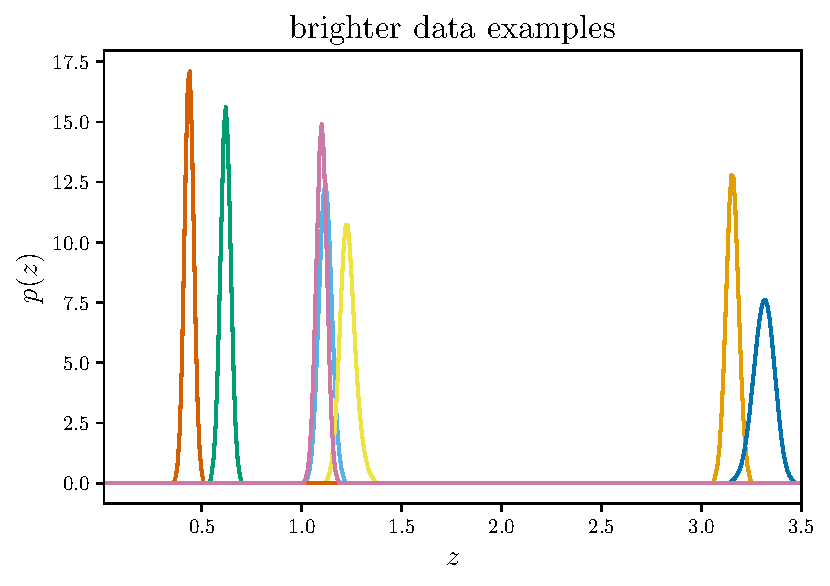
\includegraphics[width=\columnwidth]{figures/graham_pzs.pdf}
    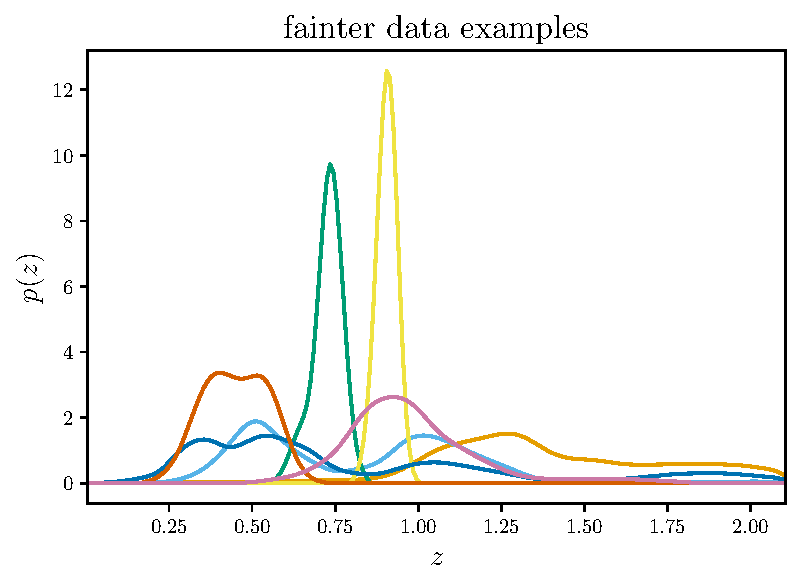
\includegraphics[width=\columnwidth]{figures/schmidt_pzs.pdf}
    \caption{
    Example \pz s from the two mock LSST datasets.
    Left: The \mgdata mock photometry yields largely narrow, unimodal \pz s.
    Right: The \ssdata mock photometry contains a higher proportion of broad 
and/or multimodal \pz s.
    \label{fig:example_pzs}}
  \end{center}
\end{figure*}

\subsection{\Mgdata data mock catalog}
\label{sec:graham}

Our first dataset is an $N_{g} = 10^{5}$ object subset of the 
\citet{graham_photometric_2017} simulated galaxy catalog used for LSST 
photometric redshift experiments.
The data builds on the Millennium simulation of large-scale structure 
\citep{springel_simulations_2005}, the galaxy formation models of 
\citet{gonzalez-perez_how_2014}, and the lightcone construction techniques of 
\citet{merson_lightcone_2013}.
The apparent $ugrizy$ magnitudes are derived from the true magnitudes using the 
aforementioned 10-year LSST errors using the software of 
\citet{connolly_end--end_2014}.
The sample is limited to galaxies with a catalog $i$-band magnitude of $i<25$ 
and true redshifts $z<3.5$, omitting any magnitudes fainter than the predicted 
10-year limiting magnitudes in each filter ($u<26.1$, $g<27.4$, $r<27.5$, 
$z<26.1$, and $y<24.9$) to realistically simulate non-detections.

The \pz\ estimates for this simulated catalog use BPZ templates based on the 
VIsible MultiObject Spectrograph Very Large Telescope Deep Survey set of 
spectra \citep{fevre_vimos_2005}, as in \citet{ilbert_accurate_2006}.
This catalog also uses the default parameter settings for BPZ with the two 
additions of a photometric redshift maximum of 3.5 and an $i$-band magnitude 
prior.
The \pz s from BPZ are in the form of $N_{ff} = 351$ evaluations of the 
probability density on a regular grid of redshifts $0.01 < z < 3.51$, a 
subsample of which are shown in the left panel of Figure~\ref{fig:example_pzs}.
As the figure shows, the \pz s from this dataset tend to be unimodal and 
sharply peaked, as if coming from brighter photometric data due to the 
conservative cuts in photometric magnitudes of this dataset.
The brighter catalog reference \pz s are three-component Gaussian mixtures fir 
to this data.

\subsection{\Ssdata data mock catalog}
\label{sec:schmidt}

Our second dataset is an independent simulation of the expected LSST galaxy 
sample, the Buzzard-highres-v1.0 mock galaxy catalog of deRose, et al.\ in 
preparation of galaxies with SEDs drawn from an empirical library of 
$\sim5\times10^{5}$ SEDs from the Sloan Digital Sky Survey (SDSS).
Given an SED, redshift, and absolute $r$-band magnitude for each galaxy, the 
$ugrizy$ magnitudes are derived from the aforementioned 10-year LSST errors.
The catalog contains $N_{g} \approx 10^{5}$ galaxies $z<2.105$ to a depth of 
$i<26.9$, 1.5 magnitudes deeper than the expected LSST gold sample of galaxies 
\citep{lsst_science_collaboration_lsst_2009}, that will have $S/N \gtrsim 30$ 
in multiple bands.

We use a custom BPZ prior using a subset of the Buzzard-highres-v1.0 catalog 
and a spanning template set via a simple k-means clustering algorithm based on 
$100$ of the SDSS SEDs used to create the Buzzard catalog.
BPZ produces \pz s in the format of probability density evaluations on a 
regular grid of $N_{ff}=211$ redshifts $0.005\leq z\leq2.105$, a subsample of 
which are plotted in the right panel of Figure~\ref{fig:example_pzs}.
The exceptional depth and known degeneracies (e.~g.~the Lyman/Balmer break 
degeneracy) lead us to expect the presence of multimodal \pz s observed in the 
figure.
The fainter catalog reference \pz s are five-component Gaussian mixtures fit to 
this data.


\section{Results \& Discussion}
\label{sec:results}

We evaluate the metrics of Section~\ref{sec:metric} on 10 random instantiations 
of catalogs of $N_{g}=100$ galaxies drawn randomly from each of the datasets 
discussed in Section~\ref{sec:data} and with each of $N_{f}=3,\ 10,\ 30,\ 100$ 
stored parameters for the three formats of Section~\ref{sec:approx}.
We then illustrate how our results could be used to choose an appropriate 
parametrization for each dataset given constraints on the distribution of KLDs 
or moment percent errors of individual \pz s, the KLD or moment percent error 
of a science metric ($\hat{n}(z)$ in this case), or the available storage 
capacity.


\subsection{Individual \pz s}
\label{sec:individual_results}

We compare our three formats on the basis of the distributions of the KLD 
calculated for every \pz\ in the dataset.
An example of an individual \pz\ KLD distribution for the \mgdata dataset with 
$N_{f}=10$ is shown in Figure~\ref{fig:individual}.
\begin{figure}
  \begin{center}
    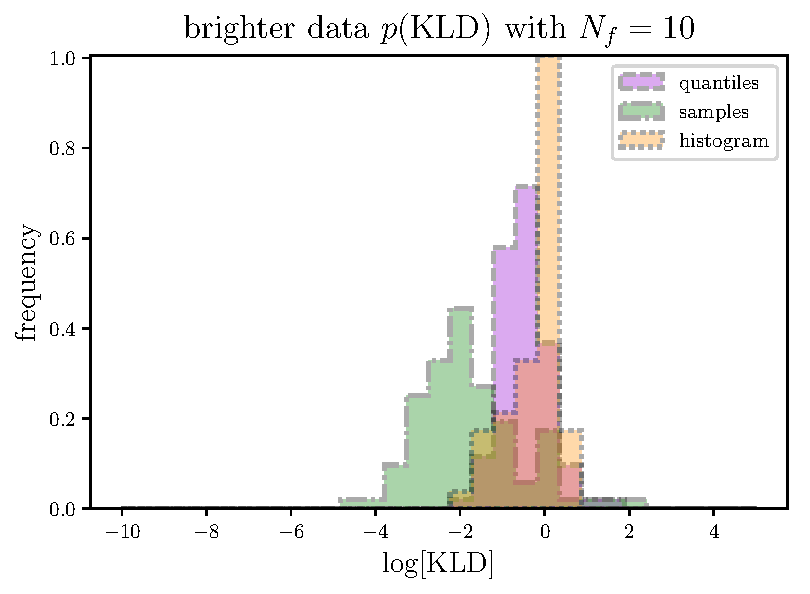
\includegraphics[width=\columnwidth]{figures/individual_kld.pdf}
    \caption{The distribution of log-KLD values for $N_{g}=100$ \pz s from the 
\mgdata dataset with $N_{f}=10$ over the quantiles (purple with dashed border), 
samples (green with dash-dotted border), and histogram (orange with dotted 
border) formats.
    In this instantiation, the samples format has a lower median KLD than the 
quantiles format, which has a lower median KLD than the piecewise constant 
format.
    Note that the distributions are over log-KLD, so the ordering of the 
formats by the breadth of the log-KLD distribution is the same as the order by 
the median.
    \label{fig:individual}}
  \end{center}
\end{figure}

To distill what is observed in the ten instantiations of plots like 
Figure~\ref{fig:individual} for both datasets and all parametrizations, we 
compare the moments of the distributions of metric values for the distribution 
of the KLDs of individual \pz s under each parametrization, summarized in 
Figure~\ref{fig:kld_moments}.
While it is obvious that one would like the mean (first moment) of the KLD 
distribution to be low, interpretation of higher-order moments is less clear.
To meaningfully interpret the KLDs of individual \pz s, it will be necessary 
for those using \pz s in their science to calculate the requirements on the 
acceptable degree of information loss.
\begin{figure*}
  \begin{center}
    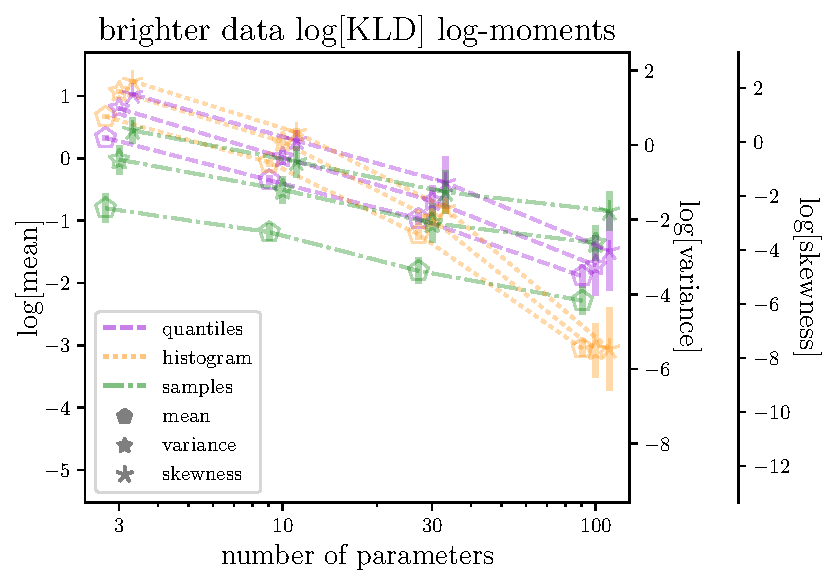
\includegraphics[width=\columnwidth]{graham_pz_kld.pdf}
    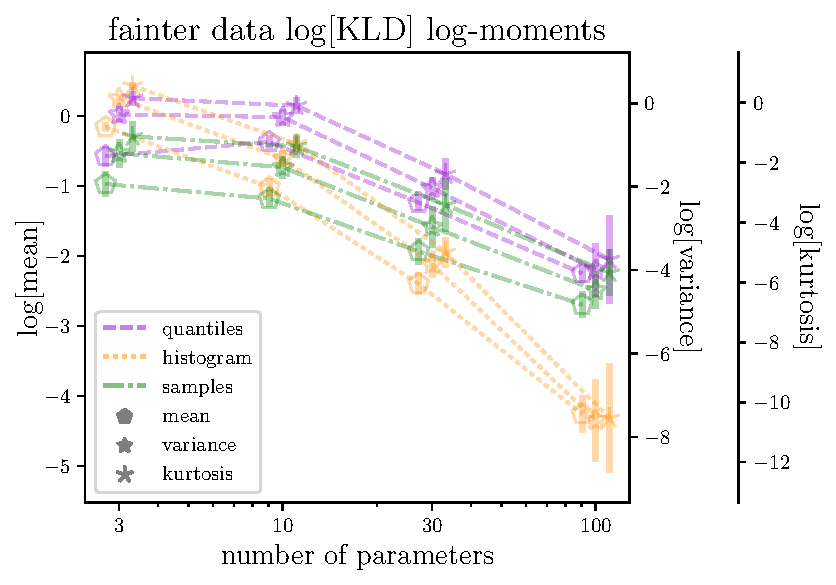
\includegraphics[width=\columnwidth]{schmidt_pz_kld.pdf}
    \caption{
    The means of the mean ($\bigstar$), variance ($+$), and kurtosis ($\times$) 
of the log-KLD distributions for each dataset as a function of the number 
$N_{f}$ of stored parameters for the quantile (dashed purple line), samples 
(dash-dotted green line), and histogram (dotted orange line) formats with 
$1\sigma$ Gaussian error bars based on 10 instantiations of 100 galaxies, which 
are offset about $N_{f}$ to improve readability.
    Left panel: The distribution of individual \pz\ KLD values of the \mgdata 
mock catalog is most well-behaved when they are stored as samples, except at 
large $N_{f}$.
    Right panel: The \ssdata mock catalog achieves equivalence of the formats 
in the moments of the log-KLD distributions at a much lower $N_{f}$, ultimately 
showing the histogram format is most well-behaved at all but the smallest 
$N_{f}$.
    \label{fig:kld_moments}}
  \end{center}
\end{figure*}

Figure~\ref{fig:kld_moments} is rich in information.
For both datasets, the behavior of the first three log-moments of the log-KLD 
distribution is highly correlated for a given format and number of parameters.
The error bars on the log-KLD log-moments increase at high $N_{f}$ for all 
formats on both datasets beyond what one would expect simply based on the log 
scaling.

The \mgdata dataset has higher log-KLD log-moments than the \ssdata dataset at 
all $N_{f}$ and across all formats, meaning information loss is enhanced for 
more strongly featured data; this observation is not surprising because the 
narrow, unimodal \pz s of the \mgdata dataset have long tails of very low 
probability that are emphasized by the KLD.
The \ssdata dataset shows almost no change in the log-KLD log-moments between 
$N_{f}=3$ and $N_{f}=10$ parameters, but both datasets otherwise exhibit a 
steady decrease in all moments for the quantile and samples formats as $N_{f}$ 
increases.

The log-KLD log-moments are higher for quantiles than for samples for both 
datasets, except at $N_{f}=100$ for the \mgdata dataset; this is not an 
unexpected result because our choice of PDF reconstruction method for the 
quantile format is most susceptible to error in the tails of the distribution, 
where the KLD has the highest sensitivity.
The histogram format's log-KLD log-moments are higher than for other formats at 
the lowest $N_{f}$ and steadily decrease in a manner similar to the other 
formats, except at the highest $N_{f}$ values where the histogram format's 
log-KLD log-moments decrease much more quickly.

We also examine the percent error on the first three moments of the \pz s under 
each approximation, using the base-10 log for interpretability.
Because the distribution of moment percent errors is highly non-Gaussian due to 
a small number ($<1\%$) of truly extreme outliers for both datasets, across all 
$N_{f}$ and all formats, we substitute the interquartile range for traditional 
$1\sigma$ Gaussian error bars.
\begin{figure*}
  \begin{center}
    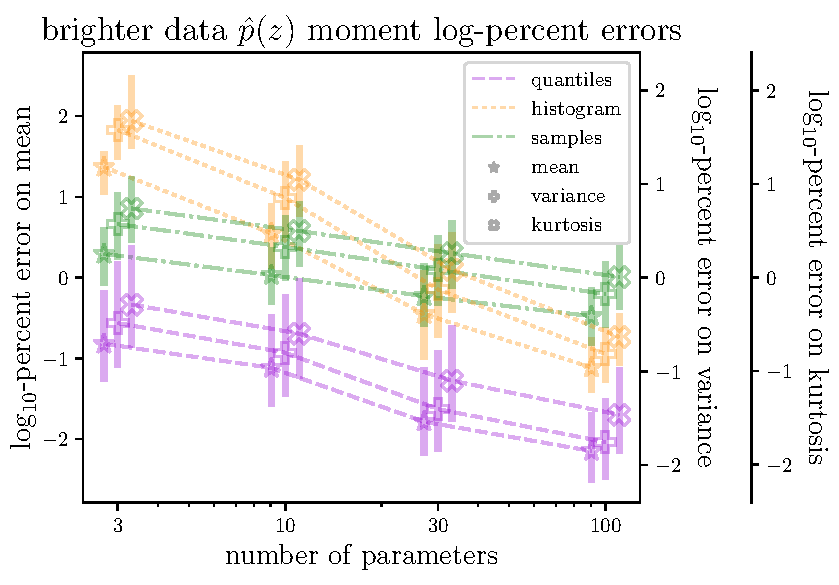
\includegraphics[width=\columnwidth]{graham_pz_err.pdf}
    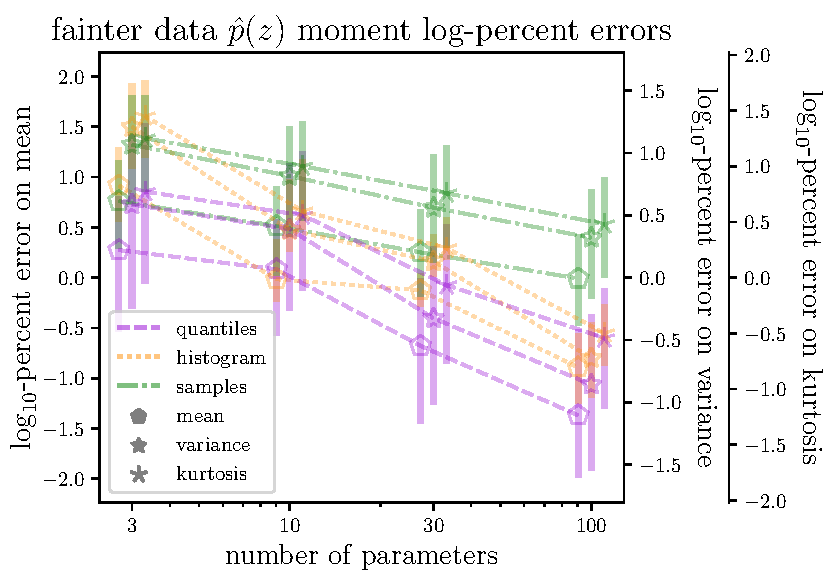
\includegraphics[width=\columnwidth]{schmidt_pz_err.pdf}
    \caption{
   The median $\log_{10}$-percent errors on the mean ($\bigstar$), variance 
($+$), and kurtosis ($\times$) of the \pz s for each dataset as a function of 
the number $N_{f}$ of stored parameters per \pz\ for the quantile (dashed 
purple line), samples (dash-dotted green line), and histogram (dotted orange 
line) formats with interquartile range error bars based on 10 instantiations of 
100 galaxies, where the $\log_{10}$-percent errors and their interquartile 
ranges are offset around $N_{f}$ to improve readability.
   Left panel: The \mgdata \pz\ ensemble's moment percent errors are minimized 
by the quantile format at all $N_{f}$.
   Right panel: The \ssdata \pz\ ensemble's moment percent errors are high for 
all formats at low $N_{f}$ but distinct at high $N_{f}$, with the quantile 
format overall outperforming the samples and histogram formats.
    \label{fig:pz_moment_errs}}
  \end{center}
\end{figure*}

Though the $\log_{10}$-percent error of the moments of individual \pz s also 
exhibits significant correlation between the moments for a given 
parametrization, the behavior is otherwise markedly different from that of the 
log-moments of the \pz\ ensemble's log-KLD distribution.
The percent errors of the moments of the approximate \pz s are overall lower in 
the \mgdata dataset than the \ssdata dataset over the same range of number of 
stored parameters; this is expected because there is simply less information to 
capture in the \mgdata dataset.

For the \mgdata dataset, the quantile format enables sub-percent errors in \pz\ 
moments at the lowest $N_{f}$, a level that cannot be achieved until $N_{f}>30$ 
parameters for the histogram format and $N_{f}>100$ for the samples format.
Furthermore, for the \mgdata dataset, the quantile format minimizes the percent 
error at all $N_{f}$, whereas the samples format outperforms the histogram 
format at low $N_{f}$ but the histogram format is outperforms the samples 
format at high $N_{f}$.
Again, this behavior is expected of the narrow, unimodal \pz s of the \mgdata 
dataset because large histogram bins are ineffective at capturing small-scale 
structure and including more samples does not significantly improve 
preservation of such features.

The ordering of the moment percent error of all formats is the same for the 
\ssdata dataset is the same as that of the \mgdata dataset at $N_{f}=3$.
In the \ssdata dataset, the inclusion of $N_{f}=30$ parameters decreases the 
moment percent error of the histogram format more significantly than the 
quantile or samples formats, to the point that the histogram and quantile 
formats have comparable moment percent errors.
At higher $N_{f}$ in the \ssdata dataset, the quantile and histogram formats 
continue to improve faster than the samples format, with the percent errors on 
the \pz\ moments being consistently lower for the quantile format than for the 
histogram format.
The broad, multimodal \pz s of the \ssdata dataset enable achievement of 
sub-percent accuracy in the moments only with $N_{f}\geq30$ under the quantile 
format and $N_{f}=100$ with the histogram format.

\subsection{Stacked $\hat{n}(z)$ estimator}
\label{sec:stacked_results}

Figure~\ref{fig:stacked} shows an example of $\hat{n}(z)$ of \pz s 
reconstructed from just $N_{f}=10$ parameters under each of our three 
approximation formats, evaluated on the same fine grid as the input \pz s.
The strong features in the curve are due to the very small sample size of $100$ 
galaxies.
As expected, the stacked histogram is quite coarse because of the step function 
interpolation, while the stacked estimator of the redshift distribution based 
on \pz\ representations that are interpolations of stored samples and quantiles 
are much closer to the stacked estimator of the original, high-resolution \pz s.
The KLD for each format is also included in the plot; in this instance, the KLD 
is lowest for the quantile format and highest for the histogram format.

\begin{figure}
  \begin{center}
    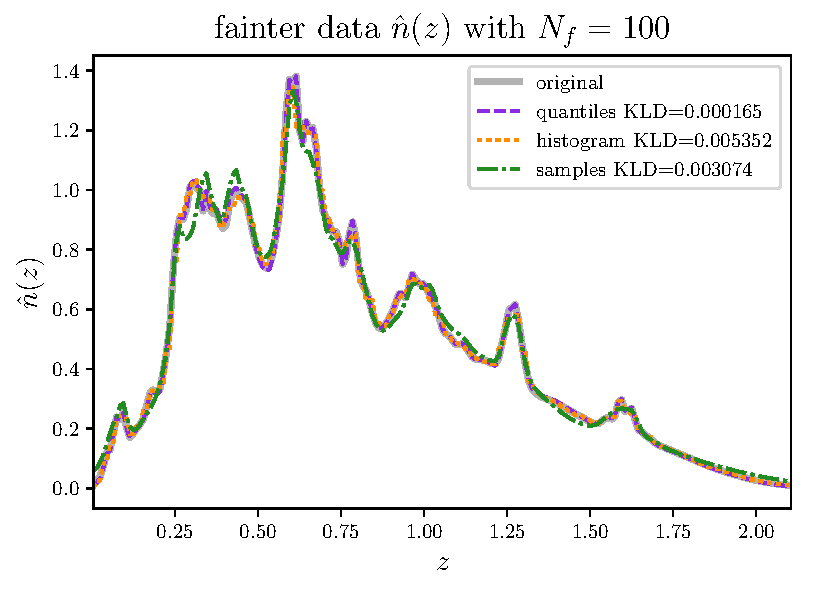
\includegraphics[width=\columnwidth]{figures/stacked.pdf}
    \caption{An example of the stacked estimator of the redshift distribution, 
for a subsample of $N_{g}=100$ galaxies drawn from the \ssdata data mock 
catalog and with $N_{f}=10$ parameters used for each \pz; the small-scale 
features are due to the small number of galaxies in the sample.
    The most striking characteristic of $\hat{n}(z)$ with a relatively small 
number of parameters on a small number of galaxies is the coarseness of the 
histogram format (orange dotted line) relative to the quantile (purple dashed 
line) and samples (green dash-dotted line) formats, both of which are fairly 
close to $\hat{n}(z)$ derived from evaluating the original, high-resolution \pz 
s (thick gray line).
    \label{fig:stacked}}
  \end{center}
\end{figure}

Again, due to the variation between $N_{g}=100$ galaxy subsamples, we repeat 
the procedure that produced Figure~\ref{fig:stacked} 10 times to generate a 
distribution over the KLD of the stacked estimator of the redshift distribution 
for each format for each dataset.
The $\hat{n}(z)$ KLD values for each parametrization on both mock datasets are 
collected and plotted in Figure~\ref{fig:kld}, with error regions based on the 
variance between the 10 instantiations.
\begin{figure*}
  \begin{center}
    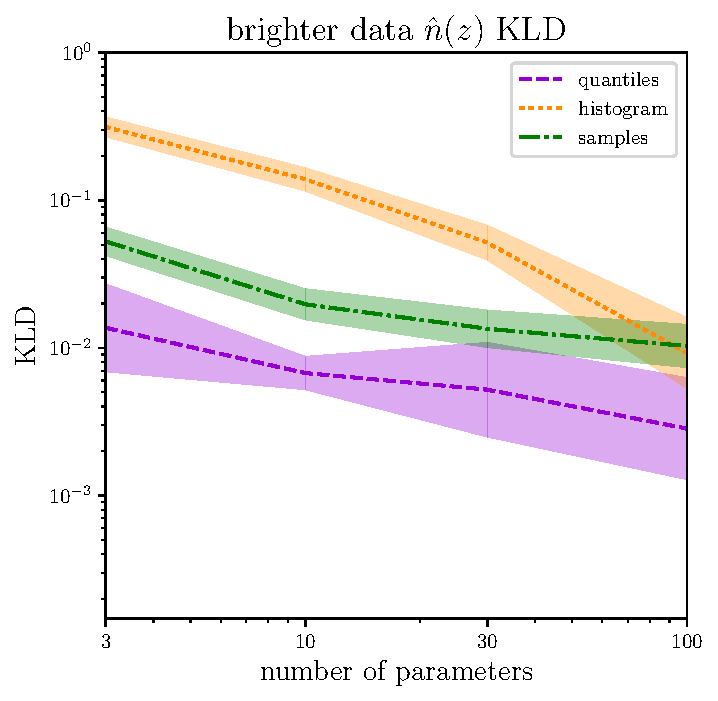
\includegraphics[width=\columnwidth]{figures/graham_nz_kld.pdf}    
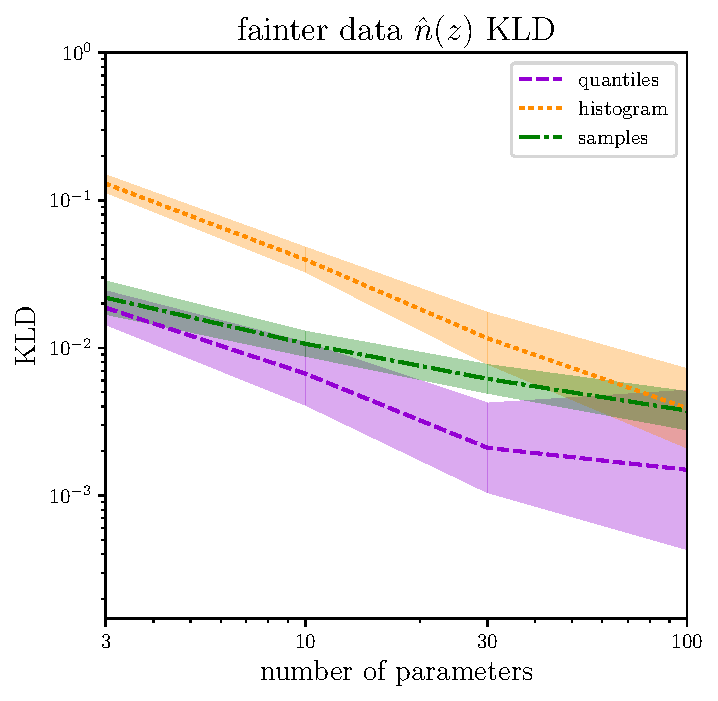
\includegraphics[width=\columnwidth]{figures/schmidt_nz_kld.pdf}
    \caption{The KLD between $\hat{n}(z)$ derived from approximate \pz\ 
representations and $\hat{n}(z)$ derived from the original, high-resolution \pz 
s, as a function of number $N_{f}$ of stored parameters, for the quantiles 
(purple dashed line), samples (green dash-dotted line), and histogram (orange 
dotted line) formats.
    Shaded regions indicate the $1\sigma$ Gaussian errors derived from 10 
subsamples of 100 galaxies and lines indicate the mean of the distribution.
    Left panel: The \mgdata \pz\ catalog's KLD of $\hat{n}(z)$ is minimized by 
the quantile format at all $N_{f}$.
    Right panel: The \ssdata \pz\ catalog's KLD of $\hat{n}(z)$ is minimized by 
the quantile format at all $N_{f}$, though the samples format also has a 
comparably low KLD.
    \label{fig:kld}}
  \end{center}
\end{figure*}
Figure~\ref{fig:kld} shows that the two datasets clearly share some features:
\begin{enumerate}
\item As expected, the KLD drops as the number of stored parameters increases, 
for all formats.
\item The quantile format minimizes the KLD at all numbers of stored parameters 
considered.  (Note that the appearance of a larger error region is due to the 
log scaling.)
\item The histogram format leads to substantial loss of information relative to 
the other formats except at large numbers of stored parameters where it is 
comparable with the samples format.
\end{enumerate}
However, there are also ways in which the behavior of the KLD on $\hat{n}$ 
differs due to the data quality's significant impact on the behavior of this 
metric:
\begin{enumerate}
\item The \ssdata dataset enables the achievement of lower KLD values than the 
\mgdata dataset for all formats at all values of $N_{f}$ considered, likely a 
consequence of the strong features present in $\hat{n}(z)$ for the \mgdata 
dataset in our subsamples of 100 galaxies.
\item The rate at which the KLD of $\hat{n}(z)$ improves with increasing $N_{f} 
$ is overall slower for the \mgdata dataset than for the \ssdata dataset; in 
other words, saving more parameters has a greater marginal benefit for the 
\ssdata dataset than for the \mgdata dataset.
\item The $\hat{n}(z)$ KLD for the samples format is not substantially higher 
than for the quantile format in the \ssdata dataset but is for the \mgdata 
dataset, which may reflect the subjectivity of the reconstruction scheme used 
for those two formats.
\end{enumerate}

We also address the relative, marginal, and absolute performance and 
consistency thereof of the KLD on $\hat{n}(z)$ for each parametrization as a 
function of format and $N_{f}$ for each dataset.
To guide this process, we interpret Figure~\ref{fig:kld} in the context of 
constraints on storage allocation imposed by the survey and constraints on the 
acceptable degree of information loss imposed by the science requirements, 
which we anticipate establishing in the future.

A constraint on storage resources corresponds to a vertical line at a given 
$N_{f, \mathrm{lim}}$ in Fig. \ref{fig:kld}; the best format would be the one 
that achieves the lowest KLD at $N_{f, \mathrm{lim}}$.
For example, if $N_{f, \mathrm{lim}}=10$ stored parameters, the quantile format 
would be optimal for the \mgdata dataset because it has the lowest KLD value by 
a large margin compared to other formats.
If the \ssdata dataset were subject to the same constraint, the quantile and 
samples formats would both be good candidates for a storage parametrization, 
with the quantile format opening the possibility of a lower KLD.
If there is some flexibility in the allocation of storage for \pz s, as is the 
case for LSST, it may be best to examine the asymptotic behavior of the KLD as 
a function of the number of stored parameters for each format considered; if 
the KLD can be significantly reduced with a slightly larger $N_{f}$, it may be 
possible to request additional storage capacity for the survey's \pz s.

A constraint on the acceptable loss of information due to compression and 
reconstruction of \pz s corresponds to a horizontal line at some 
$\mathrm{KLD}_{\mathrm{lim}}$ in Figure~\ref{fig:kld}; the best parametrization 
would correspond to the format that achieves $\mathrm{KLD}_{\mathrm{lim}}$ at 
the lowest $N_{f}$.
For example, if the brighter dataset has $\mathrm{KLD}_{\mathrm{lim}}=10^{-2}$ 
nats, the quantile parametrization with $N_{f}=3$ would be optimal due to the 
slow marginal improvement of the $\hat{n}(z)$ KLD of the quantiles and samples 
format and the high KLD for the histogram format.
If the \ssdata dataset were subject to the same constraint, the quantile 
parametrization with $N_{f}=10$ achieves $\mathrm{KLD}_{\mathrm{lim}}$ at the 
lowest $N_{f}$.



We also calculate the percent error on the moments of the stacked estimator of 
the redshift distribution, as these may be more useful for understanding error 
propagation in cosmology due to \pz\ storage parametrization than the KLD, for 
which no such infrastructure yet exists.
The percent error on the first three moments of the stacked estimator of the 
redshift distribution function is shown in Figure~\ref{fig:nz_moment_errs}.
Because the distribution of moment percent errors is highly non-Gaussian due to 
the small number of instantiations considered, we substitute the interquartile 
range for traditional $1\sigma$ Gaussian error bars.
\begin{figure*}
  \begin{center}
    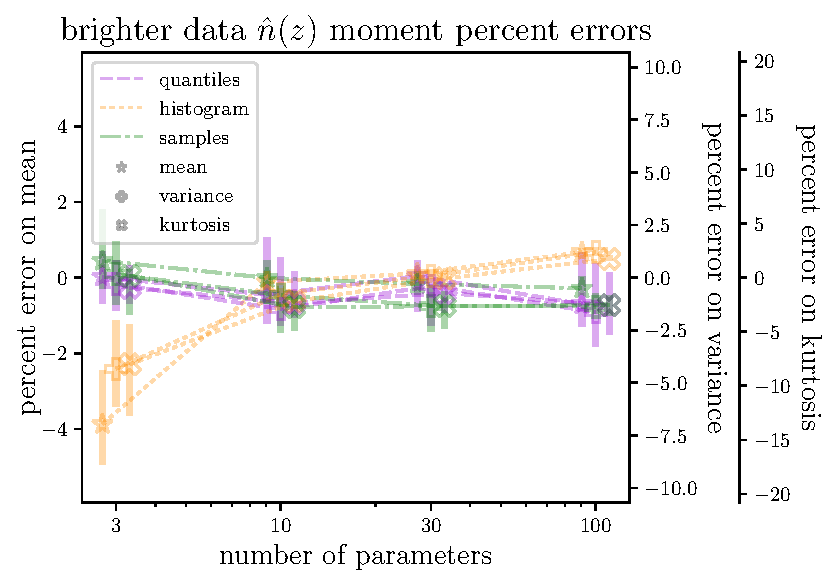
\includegraphics[width=\columnwidth]{graham_nz_err.pdf}    
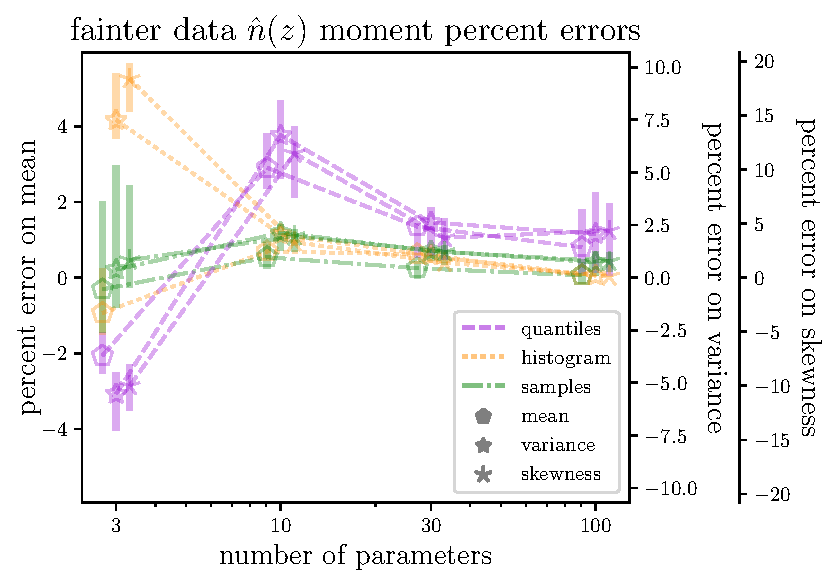
\includegraphics[width=\columnwidth]{schmidt_nz_err.pdf}
    \caption{
    The percent error on the mean ($\bigstar$), variance ($+$), and kurtosis 
($\times$) of the stacked estimator $hat{n}(z)$ of the redshift distribution 
for each dataset as a function of the number $N_{f}$ of stored parameters for 
the quantile (dashed purple line), samples (dash-dotted greenline), and 
histogram (dotted orangeline) formats with interquartile range error bars based 
on 10 instantiations of 100 galaxies, where the percent errors and their 
interquartile ranges are offset about $N_{f}$ to improve readability.
    Left panel: The \mgdata dataset shows evolution with $N_{f}$ of the 
$\hat{n}(z)$ moment percent errors for the histogram format but none for the 
samples and quantile formats.
    Right panel: The \ssdata dataset shows qualitatively different evolution 
with $N_{f}$ of the $\hat{n}(z)$ moment percent errors for the three formats 
and for each moment.
    \label{fig:nz_moment_errs}}
  \end{center}
\end{figure*}
In this metric, the significant impact of data properties is quite apparent.
To explain this, we draw the reader's attention to Figure~\ref{fig:stacked} and 
note that the actual redshift distribution for both datasets is similar, but 
the redshift range over which they are defined is larger for the \mgdata 
dataset than the \ssdata dataset.

In the \mgdata dataset, the evolution of the $\hat{n}(z)$ moment errors with 
$N_{f}$ differs for the histogram format relative to the samples and quantile 
formats.
While the samples and quantile formats exhibit essentially no evolution in 
excess of the error bars between instantiations, the histogram format 
significantly underestimates the moments at low $N_{f}$, effectively 
approximates the moment errors at intermediate $N_{f}$, and overestimates them 
at high $N_{f}$.
For $N_{f}=3$, the moments are grossly underestimated because most of the 
probability density of $\hat{n}^{r}(z)$ falls into the lowest single redshift 
bin (explaining the higher moments), and the lowest redshift bin has most of 
the probability density of $\hat{n}^{r}(z)$ above the middle of the bin 
(explaining the mean).
When the bins are too small, at $N_{f}=100$, those at high redshifts have most 
of their probability density below the middle of the bin, leading to slightly 
overestimated moments.
Because the \pz s in the \mgdata dataset are so narrow and unimodal overall, 
the reconstructions of the samples and quantile parametrizations are highly 
accurate where most of the probability density is, even with low $N_{f}$, so 
the reference representation moments are consistently recovered to within 
$<1\%$.

In the \ssdata dataset, the issues are different because the redshift range of 
the original \pz s is smaller and the \pz s themselves are broader.
The samples format has no significant evolution in moment errors with $N_{f}$, 
the histogram format severely overestimates the higher moments at low $N_{f}$, 
and the quantiles format severely underestimates the moments at low $N_{f}$, 
severely overestimates them at intermediate $N_{f}$, and moderately 
overestimates them at high $N_{f}$.
The samples format may suffer from shot noise for broad, multimodal \pz s, but 
the result is just spikier \pz s that produce narrow features in $\hat{n}(z)$ 
that do not significantly affect the moments.
The histogram format's overestimation of higher moments at low $N_{f}$ in the 
\ssdata dataset is caused by the bulk of the probability density of 
$\hat{n}^{r}(z)$ falling almost evenly into the two low redshift bins with far 
less probability in the highest bin.
As was hinted at in Figure~\ref{fig:kld_moments}, the quantile 
parametrization's \pz\ KLD distribution has large moments, and the KLD is most 
sensitive to a poor approximation of the tails of the distribution.
Both the underestimation of the $\hat{n}(z)$ moments at low $N_{f}$ and the 
overestimation of the $\hat{n}(z)$ moments at intermediate $N_{f}$ are due to 
the choice of a suboptimal reconstruction scheme for quantiles that could 
doubtlessly be improved in the future.
The quantile format's overestimation of the moments even at high $N_{f}$ can be 
explained by the fact that it is not limited to the redshift range over which 
the original \pz s were defined, a possible oversight of the \qp\ 
implementation.
A broad \pz\ may be reconstructed with probability density outside the redshift 
range of the original \pz s and then truncated and normalized prior to 
calculating the KLD.
Because broad \pz s are more likely to occur at high redshift, this excess 
probability is more likely to be at high redshift, slightly but consistently 
inflating the moments.


\section{Conclusions \& Future Directions}
\label{sec:conclusions}

This work develops a principled, systematic approach to choosing a 
parametrization for storing a catalog of \pz s from a survey of known data 
properties with a goal of balancing the available storage resources against the 
accuracy of the \pz s and science products thereof reconstructed from the 
stored parameters.
We demonstrate the recommended method on two realistic mock datasets 
representative of upcoming \pz\ catalogs and draw the following conclusions:
\begin{itemize}
  \item Some general trends are shared among the datasets we used in our tests, 
but much of the qualitative and quantitative behavior is different.
  The properties of the \pz\ catalog influence the optimal compression scheme.
  \item The parametrization that best approximates individual \pz s may differ 
from the parametrization that optimizes a given science metric.
  The science goals must motivate the metric that guides the choice of 
parametrization.
  \item In our LSST-like examples with metrics motivated by gravitational 
lensing probes of cosmology, we confirm the expectation that regular binning 
and uniform sampling in the space of probability is more effective than regular 
binning in redshift.
  This trend can only be enhanced as the quantile and sample reconstruction 
schemes improve.
\end{itemize}
To be clear, we do not advocate for a one-size-fits-all solution to the problem 
of compressing \pz\ catalogs and emphasize that any decision should account for 
the absolute, relative, and marginal behavior of the formats considered as a 
function of the number of stored parameters.

For the case of LSST, though the histogram format has the strongest presence in 
the \pz\ literature, it exhibits a higher loss of information and moment 
percent error of the reconstructed \pz s, except when a very large number of 
parameters are stored, so we do not recommend its use for LSST's \pz\ catalog.
Given the constraint that LSST will be able to store only $\sim100$ numbers to 
describe the redshift of each galaxy and intends to include the output of 
several \pz\ codes, we can safely say that LSST can store the output of more 
than one \pz\ code without risk of significant loss of information.
Had our results indicated a significant improvement in our metrics for a small 
increase in the number of stored parameters, we would present to 
decision-makers within the collaboration evidence in support of increasing that 
allocation.

Furthermore, though we discussed the previous use of each format in science 
calculations, we do not endorse the preference of any format on the basis of 
existing infrastructure for its use.
Rather, we anticipate great advances in the development of analysis techniques 
that best make use of the information in \pz s and encourage the community to 
then choose parametrizations that most effectively serve the needs of those 
intended practices.
Future analyses may also consider options we did not, such as additional 
formats, new metrics, variable $N_{f}$ over the PDF ensemble, and improved 
samples and quantile reconstruction procedures.

So that decisions of this kind can be optimized for all future surveys, the 
\qp\ Python package developed for this project is made public on GitHub as a 
tool for use by the broader community.
We invite contributions of formats, metrics, and reconstruction schemes to the 
public GitHub repository.


\subsection*{Appendix}
\label{sec:kld}

We develop some intuition for the Kullback-Leibler Divergence by contrasting it 
with the familiar metric of the root-mean-square error (RMSE)
\begin{align}
  \label{eq:rmse}
  \mathrm{RMSE} &= \sqrt{\int (P(z) - \hat{P}(z))^{2} dz}.
\end{align}
Consider the simple example of a Gaussian $P(z)=\mathcal{N}(\mu_{0}, 
\sigma_{0}^{2})$ being approximated by a Gaussian $P'(z)=\mathcal{N}(\mu, 
\sigma^{2})$, whose KLD is
\begin{align}
  \label{eq:gaussian}
  \mathrm{KLD} &= 
\frac{1}{2}\left(\log\left[\frac{\sigma^{2}}{\sigma_{0}^{2}}\right] + 
\frac{\sigma_{0}^{2}}{\sigma^{2}} + \frac{(\mu-\mu_{0})^{2}}{\sigma^{2}} - 
1\right)
\end{align}
To get a sense of the units of information, we can calculate the KLD and RMSE 
in some limiting cases.
If $\sigma=\sigma_{0}$ but $\mu=\mu_{0}+1$, we obtain 
$\mathrm{KLD}=\frac{1}{2}$ nat -- if the mean of the approximation is wrong by 
an additive factor of $\sigma$, half a nat of information is lost.
If $\mu=\mu_{0}$ but $\sigma=\sqrt{2\pi}\sigma_{0}$, we find 
$\mathrm{KLD}\approx\frac{1}{2}$ nat -- half a nat of information is also lost 
if the variance of the approximation is off by a multiplicative factor of 
$2\pi$.

We can use the KLD to identify notions of imprecision and inaccuracy.
Intuitively, precision must be related to how close $\sigma$ is to $\sigma_{0}$ 
and accuracy must be related to how close $\mu$ is to $\mu_{0}$.

\begin{figure}
  \begin{center}
    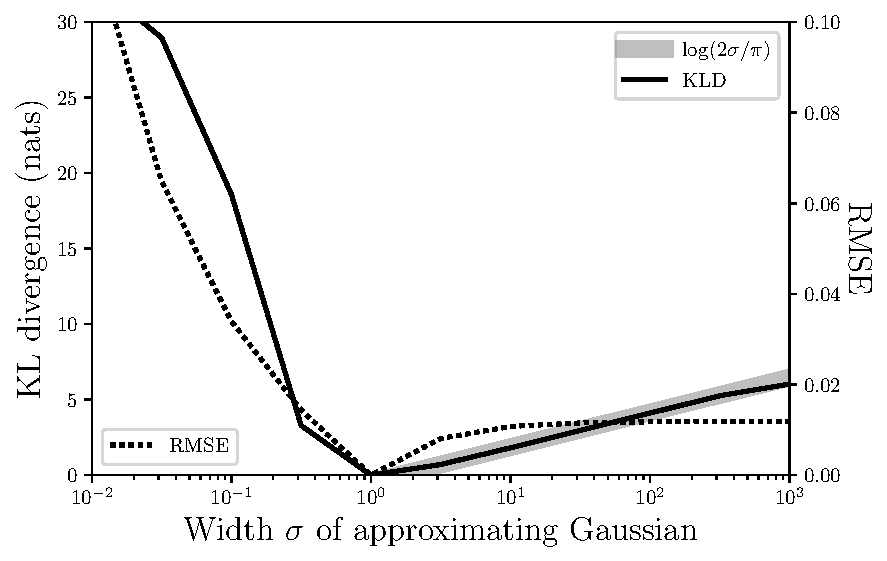
\includegraphics[width=\columnwidth]{figures/precision.pdf}
    \caption{The KLD and RMSE as a function of the root variance ratio $r$ for 
a simple Gaussian example.
    The KLD (solid line) rises sharply at $\sigma<\sigma_{0}$ and is 
proportional to the log of the inverse precision $r$ for $\sigma>\sigma_{0}$, 
behavior that is qualitatively similar to that of the RMSE (dotted line).
    \label{fig:precision}}
  \end{center}
\end{figure}

If $\mu\approx\mu_{0}$, we can say $\mathrm{KLD}\sim\log[r] + \frac{1}{2}r^{-2} 
- \frac{1}{2}$ where $r^{-1}\equiv\frac{\sigma_{0}}{\sigma}$ is a measure of 
\textit{precision}, whose behavior is illustrated in 
Figure~\ref{fig:precision}, alongside that of the RMSE.  We observe that an 
overestimated variance increases the KLD as the log of the square root of the 
ratio of the estimated variance to the true variance.

\begin{figure}
  \begin{center}
    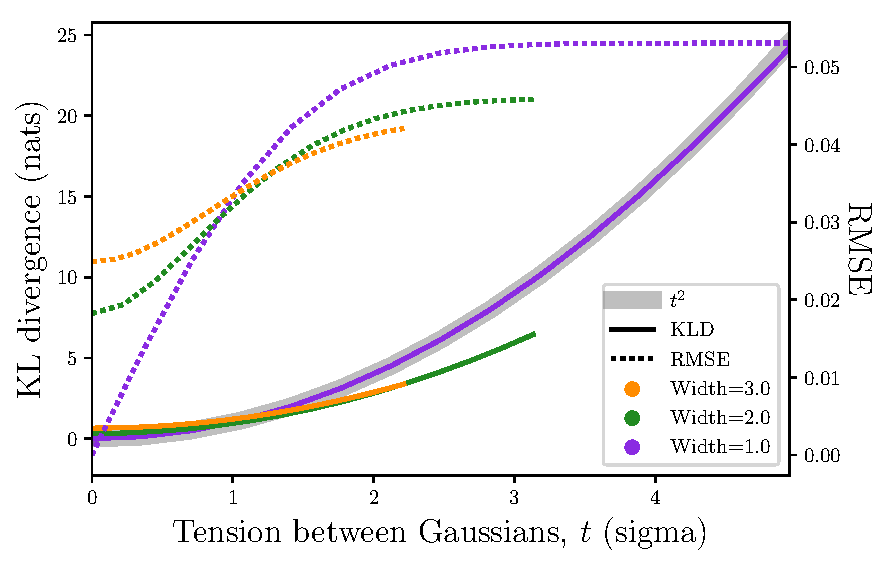
\includegraphics[width=\columnwidth]{figures/tension.pdf}
    \caption{The KLD and RMSE as a function of the tension $t$ for a simple 
Gaussian example.
    The KLD (solid lines) is equal to the square of the tension $t$, with a 
small offset when $r\neq1$, whereas the RMSE (dotted lines) is relatively 
insensitive to tension past a certain point but more sensitive to $r\neq1$.
    \label{fig:tension}}
  \end{center}
\end{figure}

When $\sigma\approx\sigma_{0}$, $\mathrm{KLD}\sim t^{2}$ in terms of the 
\textit{tension} $t\equiv\frac{(\mu-\mu_{0})^{2}}{\sigma^{2}}$, whose 
concordance is illustrated in Figure~\ref{fig:tension}.
There is some limiting tension $t_{\mathrm{lim}}\approx2$ below which the RMSE 
is more sensitive than the KLD and above which the KLD is more sensitive than 
the RMSE.
This behavior hints at the KLD's reputation for sensitivity to the tails of a 
distribution.
The notion of tension may be more important for cosmological applications of 
\pz s, indicating the KLD may be a more appropriate metric for coarser 
approximations and the RMSE may be a more appropriate metric for less coarse 
approximations.

\subsection*{Acknowledgments}


This work was incubated at the 2016 LSST-DESC Hack Week hosted by Carnegie 
Mellon University.
AIM is advised by David Hogg and was supported by National Science Foundation 
grant AST-1517237.
The work of AIM was also supported by the U.S. Department of Energy, Office of 
Science, Office of Workforce Development for Teachers and Scientists, Office of 
Science Graduate Student Research (SCGSR) program, administered by the Oak 
Ridge Institute for Science and Education for the DOE under contract number 
DE‐SC0014664.
The work of PJM was supported by the U.S. Department of Energy under contract 
number DE-AC02-76SF00515.
SJS was partially supported by the National Science Foundation under grant 
N56981CC.

%
%This is the text imported from \code{acknowledgments.tex}, and will be replaced by some standard LSST DESC boilerplate at some point.
%


We would like to thank Chad Schafer, Chris Morrison, Boris Leistedt, Stefano 
Cavuoti, and Maciej Bilicki for helpful feedback in the preparation of this 
paper.
AIM thanks Coryn Bailer-Jones, Eric Ford, and Morgan Fouesneau for helping to 
provide context for this work outside cosmology.

Author contributions are listed below. \\
A.I.~Malz: Initiated project, led development work. \\
P.J.~Marshall: Advised on statistics, and project design and management. \\
S.J.~Schmidt: Produced the PDFs for the fainter mock catalog. \\
M.L.~Graham: Produced the photometry and PDFs for the brighter mock catalog. \\
J.~DeRose: Produced the photometry for the fainter mock catalog. \\
R.~Wechsler: Supervised production of the fainter mock catalog. \\



\bibliography{lsstdesc,main}

\end{document}
